\documentclass[11pt]{article}

\usepackage[margin=1in]{geometry}
\usepackage{fancyhdr} % Custom headers and footers
\pagestyle{fancy}
\usepackage[T1]{fontenc} % Use 8-bit encoding that has 256 glyphs
\usepackage{fourier} % Use the Adobe Utopia font for the document - comment this line to return to the LaTeX default
\usepackage[english]{babel} % English language/hyphenation
\usepackage{amsmath,amsfonts,amsthm,amssymb} % Math packages
\usepackage{graphicx} %Add graphics to work
\usepackage[font=small,labelfont=bf]{caption} % Required for specifying captions to tables and figures
\usepackage{subcaption}
\usepackage{lipsum} % Used for inserting dummy 'Lorem ipsum' text into the template
\usepackage{float}
\usepackage{verbatim}
\usepackage{graphicx}
\graphicspath{C:/Users/nacho/Documents/School/Ph22/}
\usepackage{sectsty} % Allows customizing section commands
\allsectionsfont{\flushleft\normalfont\scshape} % Make all sections centered, the default font and small caps

\lhead{Ph22 - Assignment 2}
\chead{Daniel Chica}
\rhead{\today}

\begin{document}
	\title{Ph22- Assignment 2}
	\author{Daniel Chica}
	\date{\today}
	\maketitle

\noindent\rule{6.5in}{0.5pt}
\section*{\huge Problem 2}
\rule{6.5in}{2pt}\\
To begin, I used the same parsing function I wrote for the last assignment. This function allows me to input a string representing a function (written as if under NumPy) and let's me evaluate the function. Then I wrote functions for a forward Euler and a Midpoint method to approximate the value of a function after some step h. For the Euler, we need an expression for the derivative of the function. For the Midpoint method this is not necessary. I iterated each function 10 times and plotted how the Global Error changes as we performed each iteration for $f= \frac{1}{10} t^{2}$.

\begin{figure}[hb]
\begin{center}
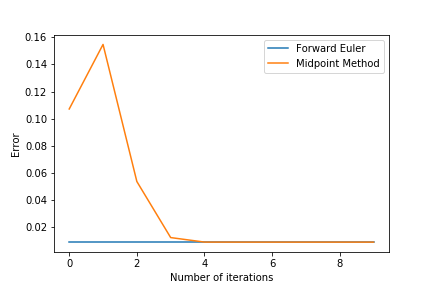
\includegraphics[scale=.6]{Error1.png}
\end{center}
\caption{Error value per iteration.}
\end{figure}\\

\noindent We see here that the Midpoint method tends to deviate a decent amount while the Euler method returns very little error compared to the actual value almost from the beginning. I found this peculiar since I expected the Midpoint method to result in a smaller error convergence than that for the Euler method. However, depending on the function I introduced, the value of the function tended to explode so it might be possible that it flies to infinity the same way the newton-Raphson method does depending on the function.\\
\noindent\rule{6.5in}{0.5pt}
\pagebreak
\section*{\huge Problem 3}
\rule{6.5in}{2pt}

\begin{figure}[hb]
\begin{center}
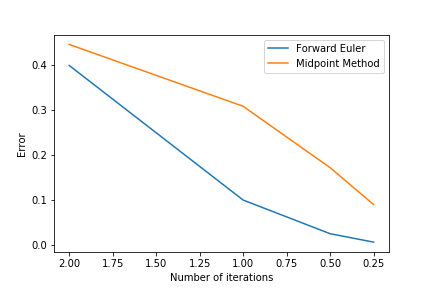
\includegraphics[scale=.6]{Error2.png}
\end{center}
\caption{Error value as h changes.}
\end{figure}\\

\noindent Here I used the same functions, but instead of iterating them, I just plotted how the error changes as we make the step size h smaller. I flipped the x-axis so that we see how the error gets smaller and smaller for both cases as we decrease the value of the step size. I began with an initial value of $h=2$, and divided the step size in half very time until reaching $h=\frac{2}{16}$. Once again the Euler method converged quicker, likely for the same reasons as before since I used the same function $f= \frac{1}{10} t^{2}$.

\noindent\rule{6.5in}{0.5pt}
\pagebreak

\section*{\huge Problem 5}
\rule{6.5in}{2pt}\\
\begin{figure}[hb]
\begin{center}
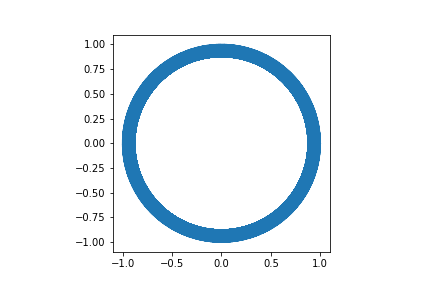
\includegraphics[scale=.6]{RKorbit.png}
\end{center}
\caption{Orbit found using Runge-Kutta routine.}
\end{figure}

\noindent Initially, I have to determine the value of R and set the forces equal to one another. Since we want a circular orbit, I decided to set $R=1$ and made it constant since it will not change over time.This led to the equation $1=x^{2}(t)+y^{2}(t)$.  I also set the initial $v=0$ for the final step so that the equations matched, and this allowed the forces on both side to equal
\begin{eqnarray*}
\frac{v^{2}}{R} = \sqrt{v'^{2}_{x}(t)+v'^{2}_{y}(t)}\\
v^{2} = \sqrt{x^{2}(t)+y^{2}(t)}\\
v = \sqrt{x^{2}(t)+y^{2}(t)}\\
1 = x^{2}(t)+y^{2}(t)\\
\end{eqnarray*}

This allows me to parametrize the equation as
\begin{eqnarray*}
x(t) = Cos(t)\\
y(t) = Sin(t)\\
\end{eqnarray*}

I plugged both these equations into the routine for a range of t and plotted the results. Sure enough, we see circular orbit about the center, reminiscent of the orbit we expect from this system of equations.
\noindent\rule{6.5in}{0.5pt}
\end{document}